\section{Results, Analysis and Discussion}
\label{sec:results}

% Numbers come from 8_Results/analysis/out (make all); figures from
% tools/make_results_figs.py.

\subsection{Proposed Solution}
\label{sec:solution}
The delivered system (\cref{fig:device}) is a self-contained power shuffler for a three-module string: one Version 0 PCB carrying two interleaved buck-boost shufflers, the NUCLEO-G474RE that closes the loop, and a Raspberry Pi pod with an LCD, an RGB LED and an IR receiver, in a printed enclosure with a heatsink. Against the objectives, the $N$-module averaged model gives the plant and its DC gain in closed form (\cref{sec:analytical}); the decoupling MIMO controller is written once in C and runs unchanged in SIL, in QSPICE and in the firmware; the controller board senses the four winding currents and the module voltages; and the system was validated on the bench and on a real string in the sun. In use, the operator picks a preset with the IR remote or the parameter page, the firmware soft-starts the legs and closes the loop, and the module-voltage differences and circulating currents are held at zero while Grafana shows the live telemetry. Any trip latches FAULT with the legs switched off.

\begin{figure}[htbp]
  \centering
  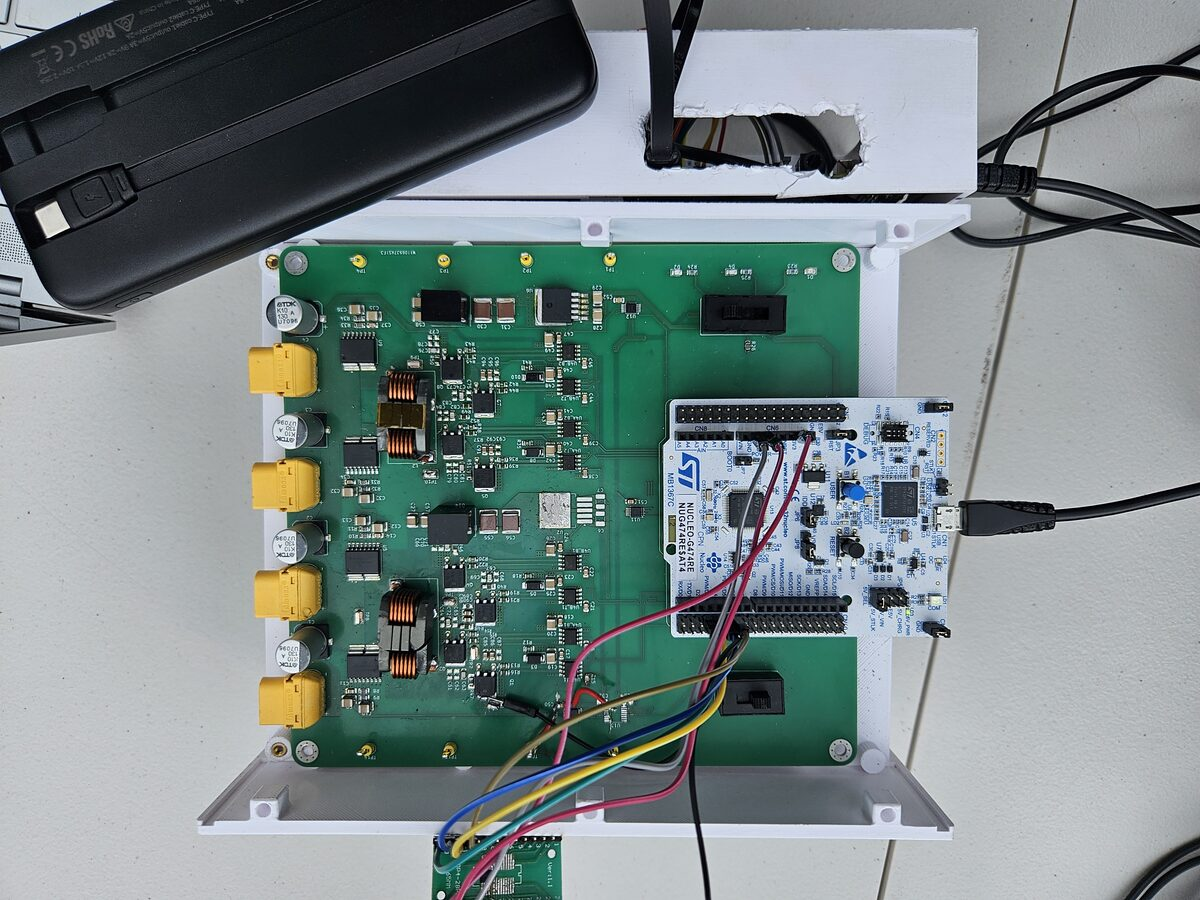
\includegraphics[height=5.0cm]{20261020_112730}
  \caption[{The built power shuffler on 20 Oct 2026}]{The built power shuffler on 20 Oct 2026: PCB, Nucleo, Pi pod, LCD and heatsink (the CAD render is on the title page).}
  \label{fig:device}
\end{figure}

\subsection{Analytical}
\label{sec:res_analytical}
The analytical $N=3$ model sets the expectation for every later phase. \Cref{tab:G} reads its DC gain as what one per cent of duty does. On every plant and in every model, 1\,\% of common-mode duty moves the voltage difference by about 0.4\,V, close to $\Vbar/100$, because $Z_e \gg R_m$ (\cref{sec:analytical}). The current block is where the plants differ. With averaged switches, 1\,\% of differential-mode duty moves the circulating current by 6.7\A; once the switching resistance is included it is 1.4\A{} at 200\,kHz and 0.24\A{} at 400\,kHz. The gain identified in QSPICE on the bench operating point (1.43 / 1.39\A) sits within 13\,\% of the analytical bench value (1.61\A), which is the evidence that $R_{sw}$ is real. The averaged Simulink plant over-estimated the current-loop gain fivefold (7.42\A), and its gain set was rejected for the hardware. The last column of \cref{tab:G} is the one term the averaged model cannot predict: a 0.14--0.25\V{} cross-coupling from differential-mode duty into $\vd{}_{,1}$, caused by the dead time, which the identified gain matrix cancels.

% generated by tools/make_tables.py -- do not edit by hand
\begin{table}[htbp]\centering
\footnotesize
\caption[{DC gain matrix $G(N)$ read as ``what 1\,\% of duty does''}]{DC gain matrix $G(N)$ read as ``what 1\,\% of duty does'': the voltage block (common-mode duty $u_c$ to the voltage difference $v_d$) and the current block (differential-mode duty $u_d$ to the circulating current $i_c$), shuffler 1 / shuffler 2 where they differ. The last column is the dead-time cross-coupling that only the switching model shows. The gain sets store $M = G^{-1}\mathrm{diag}(k_I)$, so $G = \mathrm{diag}(k_I)\,M^{-1}$.}\label{tab:G}
\begin{tabular}{l l r r r}
\toprule
Obtained from & Plant & \makecell[r]{$\Delta v_d$ [V] per\\1\,\% of $u_c$} & \makecell[r]{$\Delta i_c$ [A] per\\1\,\% of $u_d$} & \makecell[r]{cross: $\Delta v_{d1}$ [V]\\per 1\,\% of $u_{d1}$} \\
\midrule
Analytical & Solar string, averaged switches ($R = 61$\,m$\Omega$) & -0.40 & 6.72 & 0.00 \\
Analytical & Solar string, 200\,kHz ($R_{sw} = 0.29\,\Omega$) & -0.38 & 1.41 & 0.00 \\
Analytical & Solar string, 400\,kHz ($R_{sw} = 1.72\,\Omega$) & -0.29 & 0.24 & 0.00 \\
Analytical & Bench supplies in current limit, 200\,kHz & -0.47 & 1.61 & 0.00 \\
Simulink step tests & Bench, averaged switches (rejected) & -0.46 / -0.47 & 7.42 / 7.42 & -0.01 \\
QSPICE step tests & Bench, 200\,kHz (deployed) & -0.46 / -0.47 & 1.43 / 1.39 & -0.25 \\
QSPICE step tests & Bench, 300\,kHz (deployed) & -0.45 & 0.59 / 0.57 & -0.17 \\
QSPICE step tests & Bench, 400\,kHz (deployed) & -0.42 / -0.43 & 0.23 & -0.14 \\
\bottomrule
\end{tabular}
\end{table}


The root locus (\cref{fig:ana_rl}, \cref{app:analytical}) shows the margin of the deployed gains. With the deployed $M$, the voltage-loop poles stay real up to $k \approx 1$ and the circulating-current loops become complex first. The same $M$ on the 61\,m$\Omega$ averaged plant crosses into the right half-plane near $k \approx 1.5$, a second reason the averaged gain set could not be used. The open-loop phase portraits (\cref{fig:ana_portraits}) show the same trend: as the plant resistance grows with $\fsw$, the voltage mode changes from a lightly damped focus to an over-damped node.
\subsection{Simulink}
\label{sec:res_simulink}
The MIL model passed all seven validation tests (\cref{tab:validate}, \cref{app:simulink}). \Cref{fig:twin_sim} shows the carpark twin, which adds the sensing model, closing the loop on the three-module solar plant. In (a) a $+1\V$ step on the $\vd{}_{,2}$ reference is followed with the first-order shape of the design, with $\tau$ of 11.6, 3.5 and 0.56\ms{} at $k = 0.1$, 0.3 and 1 against the design 10.6, 3.5 and 1.06\,ms, while $\vd{}_{,1}$ does not move: the voltage loops are decoupled. In (b) and (c) module 3 loses a third of its irradiance. In open loop at $D = 0.5$ the shufflers already carry most of the deficit but leave a residual $\vd = -R_m\im$ of 0.06 and 0.12\V; the closed loop removes it within 15\ms{} at $k = 0.3$. Panel (c) shows why the string recovers: the shuffled currents step to 0.97 and 1.92\A, the weighted sums of the mismatch predicted by $T^{-1}\delta I$ (0.96 and 1.92\,A), and the string current settles at the mean module current, 3.82\A. The only overshoot in the twin is on the bench plant at $k=1$ (8.8\,\%).

\begin{figure}[htbp]
  \centering
  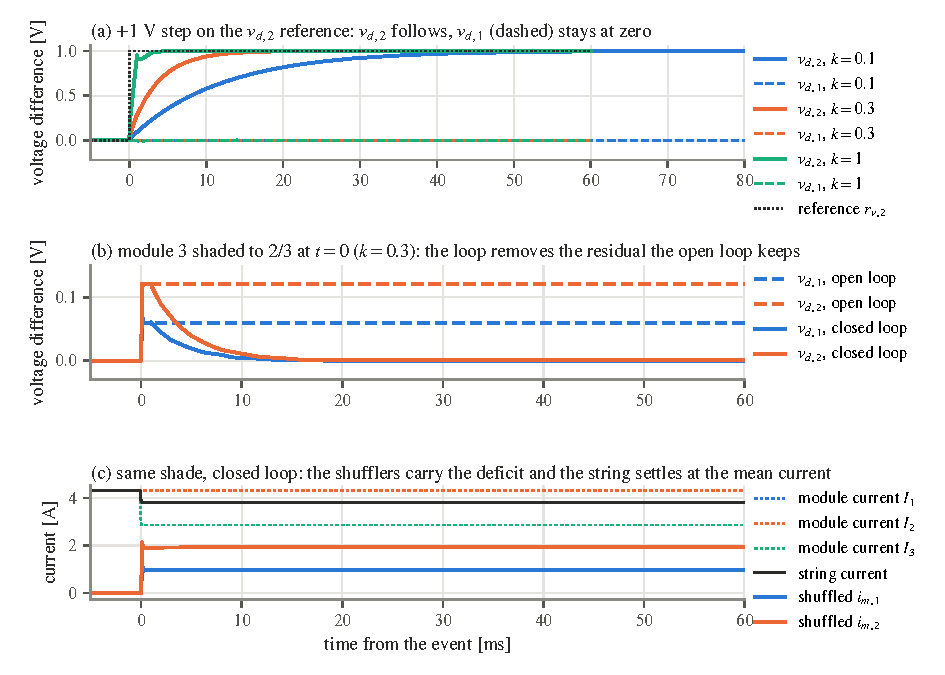
\includegraphics[width=\linewidth]{results/twin_sim}
  \caption[{Simulink carpark twin (averaged switches, sensing model, solar plant)}]{Simulink carpark twin (averaged switches, sensing model, solar plant): (a) $+1\V$ reference step at three gain scales, (b, c) module 3 shaded to two thirds at $t=0$, closed loop against open loop.}
  \label{fig:twin_sim}
\end{figure}

\subsection{QSPICE}
\label{sec:res_qspice}
\Cref{fig:qspice_run} is the strongest simulated evidence, because it runs the unchanged firmware control core as a DLL against real switches, drivers, dead time and the sensor models. A single run at $k = 0.3$ on the solar plant closes the loop on the open-loop residual, follows a $+1\V$ step on the $\vd{}_{,2}$ reference with $\vd{}_{,1}$ held, and then rejects a shade on module 3. The shuffled currents pick up the mismatch, the circulating currents stay within $\pm0.1\A$, and the string current falls to the mean module current.

\begin{figure}[htbp]
  \centering
  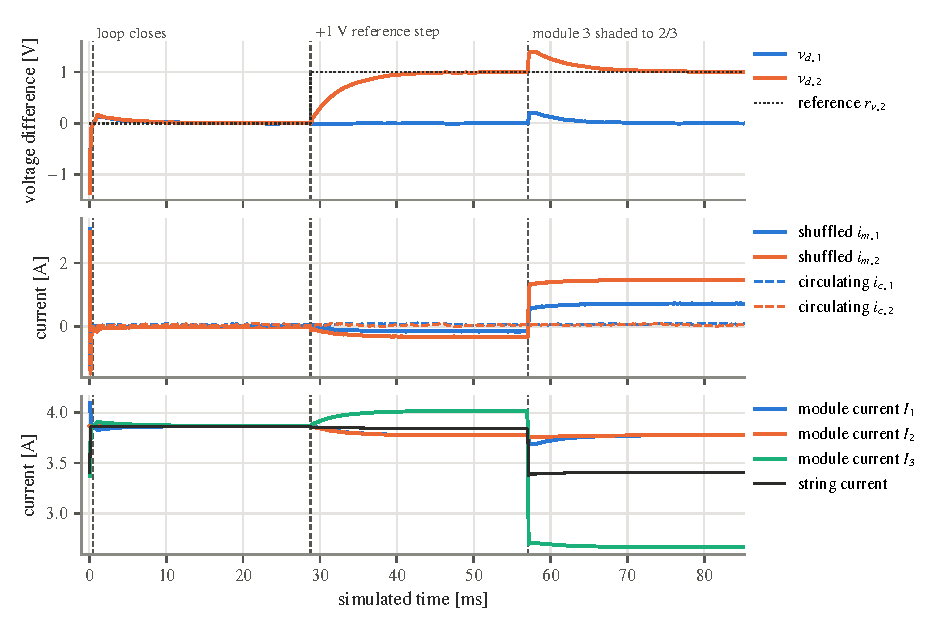
\includegraphics[width=\linewidth]{results/qspice_run}
  \caption[{QSPICE switching model with the firmware control DLL, solar plant, $k=0.3$}]{QSPICE switching model with the firmware control DLL, solar plant, $k=0.3$ (100\,$\mu$s bin means of the switching waveforms): loop closure, $+1\V$ reference step on $\vd{}_{,2}$, then module 3 shaded to two thirds.}
  \label{fig:qspice_run}
\end{figure}

The 200\,kHz gain matrix identified from this model, and deployed on the hardware, is
\begin{equation}
  G_{200} \;=\;
  \begin{array}{r@{\;}c}
   & \begin{array}{rrrr} \;\;u_{c1} & \;\;u_{c2} & \;\;u_{d1} & \;\;u_{d2} \end{array}\\[2pt]
  \begin{array}{r} v_{d1}\\ v_{d2}\\ i_{c1}\\ i_{c2} \end{array} &
  \left[\begin{array}{rrrr} -46.3 & -0.2 & -24.7 & -0.1\\ -0.2 & -46.9 & -0.1 & -27.4\\ -1.1 & -0.3 & 142.5 & 1.4\\ -1.4 & -0.9 & 0.1 & 139.0 \end{array}\right]
  \end{array}
  \label{eq:G200}
\end{equation}
in volts or amperes per unit duty. Its structure is the analytical one: a voltage block of $-\Vbar \approx -46.6\V$ with neighbour terms below 0.5\,\%, a current block of $\Vbar/R_c$, and almost no current response to the common-mode duty. The only new terms are the $\vd/\ud$ cross terms of $-25$ and $-27\V$, the dead-time effect. The matrix is well conditioned (cond$\,G = 3.2$), so its inverse, the stored gain matrix $M$, is well behaved (\cref{app:gains}).

The device model also reproduces the switching ripple (\cref{tab:T6}). QSPICE matches $\Delta\ic = \Vbar/(2\fsw(L+M))$ to within 1--3\,\% at all three frequencies. Each winding carries half of the circulating ripple, and in the shuffled current the two interleaved windings cancel, leaving only 0.2--0.4\,A. Had the circulating mode seen $L-M$ instead, the ripple would be 28--57\,A, so this result also confirms the as-built anti-series coupling. The telemetry cannot see the ripple: its samples are box-averaged over a whole control tick, and their spread is sensing noise. QSPICE was not used to judge milliamp and millivolt levels of $\ic$ and $\vd$, which depend on milliohm parasitics and nanosecond edges.

% generated by tools/make_tables.py -- do not edit by hand
\begin{table}[htbp]\centering
\small
\caption[{Peak-to-peak switching ripple: analytical against QSPICE}]{Peak-to-peak switching ripple in A. The circulating mode sees $L+M$, so the analytical law is $\Delta i_c = \bar V/(2 f_{sw}(L+M))$ with $L+M = 13.75\,\mu$H and $\bar V = 46.6$\,V. Each winding carries half of it ($\Delta i_A$); in the shuffled current the two interleaved windings cancel ($\Delta i_m$). The 44\,Hz telemetry cannot see the ripple: its $\sigma(i_c)$ is sensing noise.}\label{tab:T6}
\begin{tabular}{r r r r r r r}
\toprule
$f_{sw}$ [kHz] & \makecell[r]{$\Delta i_c$\\analytical} & \makecell[r]{$\Delta i_c$\\QSPICE} & \makecell[r]{$\Delta i_A$ per\\winding} & \makecell[r]{$\Delta i_m$\\QSPICE} & \makecell[r]{QSPICE vs\\analytical} & \makecell[r]{telemetry\\$\sigma(i_c)$} \\
\midrule
200 & 8.47 & 8.39 & 4.25 & 0.19 & -1\,\% & 0.30 \\
300 & 5.65 & 5.58 & 2.85 & 0.20 & -1\,\% & 0.05 \\
400 & 4.24 & 4.09 & 2.18 & 0.39 & -3\,\% & 0.08 \\
\bottomrule
\end{tabular}
\end{table}


\subsection{Bench Testing}
\label{sec:bench}
Bench testing was a success. The set-up was the three-channel supply (NGE103), the electronic load (DL3021), an oscilloscope, a laptop and the full system (\cref{tab:setup}). Testing started at 200\,kHz in open loop to get the baseline behaviour, then closed the loop at 0.1, 0.2 and 0.3 of the QSPICE gains, then ran 300\,kHz at 0.3 and 0.5 and 400\,kHz at 0.3. 300\,kHz was the most favourable: as the switching frequency rises the open-loop residual and the current-loop gain fall, but the heatsink temperature rises (\cref{app:thermal}). An open-loop test at 100\,kHz was also explored on 13 Oct; the system ran, but with erratic behaviour. The supplies cannot deliver as much as the panels, so the bench exercised the loop rather than the power stage.

\textbf{Open loop.} The three open-loop duty steps (\cref{fig:S5}, \cref{tab:T3duty} in \cref{app:bench}) confirm the model's DC gain on hardware: every measured change in $\vd$ is within 0.02\,V of $-\Vbar\Delta\uc$, and the shuffler whose duty did not change stays put. At duties of 0.5 the residual $\vd{}_{,2}$ is $-0.17\V$ at 200\,kHz, $-0.58\V$ at 300\,kHz and $-0.94\V$ at 400\,kHz (\cref{tab:T2ol}). This is the $-R_m\im$ drop, growing with $R_{sw}$, that the closed loop has to remove.


\begin{figure}[htbp]
  \centering
  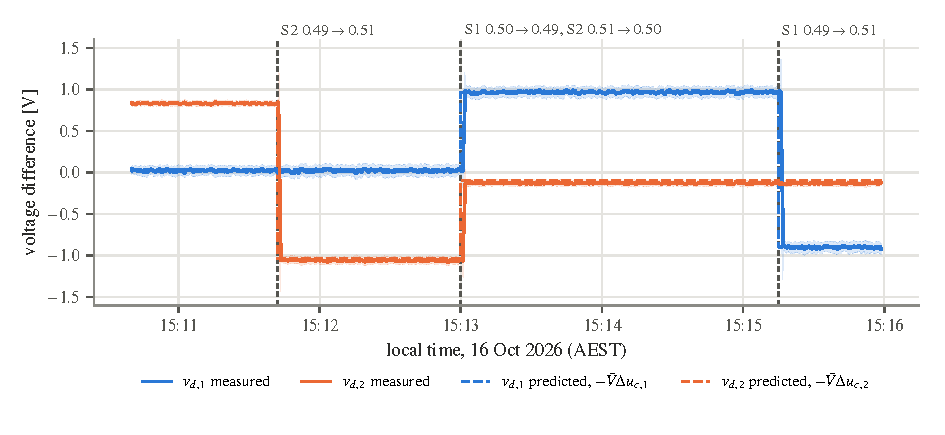
\includegraphics[width=\linewidth]{results/duty_steps}
  \caption[{Open-loop duty steps on the bench (16 Oct, 200\,kHz)}]{Open-loop duty steps on the bench (16 Oct, 200\,kHz): measured voltage differences (1\,s mean, $\pm1\sigma$ band) against the averaged-model prediction $-\Vbar\Delta\uc$ (dashed), which overlays the measurement.}
  \label{fig:S5}
\end{figure}

\textbf{Closed loop.} \Cref{fig:B06} shows 300\,kHz at $k = 0.3$ through seven step changes of the supply channels. The shuffled currents move to carry each new mismatch while the 1\,s means of both voltage differences stay within $\pm0.008\V$ and of both circulating currents within $\pm0.03\A$; the raw samples scatter by 0.016\V{} and 0.055\A. Over all 22 settled closed-loop segments, $|\bar v_{d,2}| \le 0.010\V$ and $|\bar\imath_{c,2}| \le 0.066\A$, with sample noise $\sigma(\vd{}_{,2})$ of 0.013--0.17\V{} (\cref{tab:T2cl}): the references are held with no measurable offset, and the residual is sensing noise. The 150\,ms soft-start leaves 0--0.8\,V on $\vd{}_{,2}$, which the loop removes within one telemetry frame in 10 of 23 closures and within 3\,s, limited by noise, in the rest (\cref{tab:T3close}).

\begin{figure}[htbp]
  \centering
  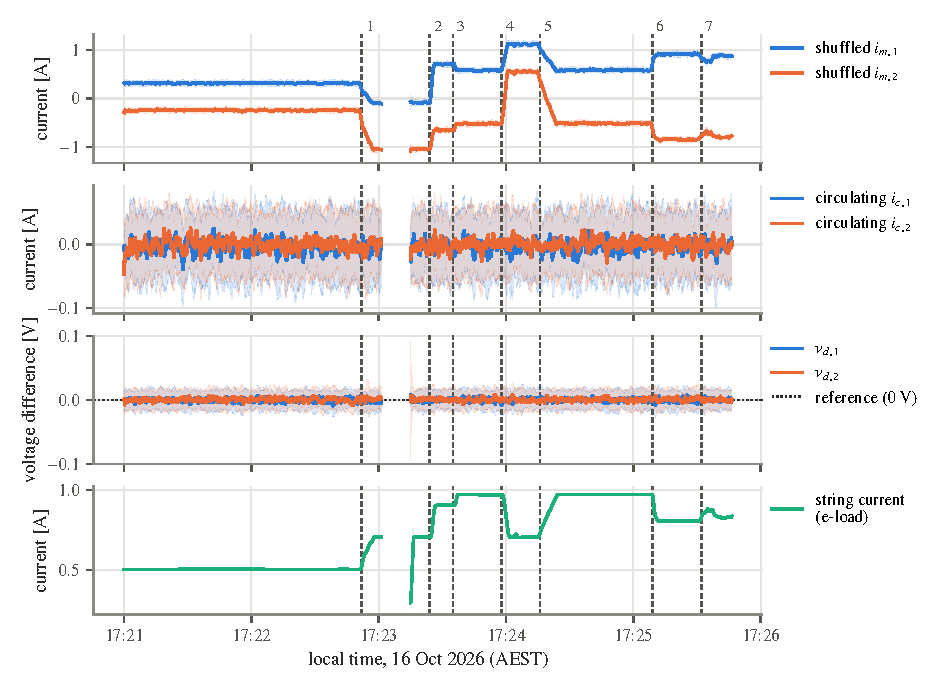
\includegraphics[width=\linewidth]{results/bench_B06}
  \caption[{Bench, 300\,kHz closed loop, $k=0.3$ (B06)}]{Bench, 300\,kHz closed loop, $k=0.3$ (B06): 1\,s means with the $\pm1\sigma$ spread of the 44\,Hz samples. The dashed lines 1--7 are step changes of the supply channels; the shuffled currents move, the voltage differences and circulating currents do not.}
  \label{fig:B06}
\end{figure}

\textbf{Stability limit and faults.} At 300\,kHz and $k = 0.6$ the loop oscillated ($\sigma(\vd{}_{,2}) = 1.41\V$, 11.8\,V peak to peak) for 6\,s before it was stopped, so the 300\,kHz gain set loses margin above $k \approx 0.5$. Applying a new gain scale while the loop was running tripped the firmware three times (\cref{tab:T3kscale}): once on module under-voltage and twice on a main-loop stall. Each trip switched the legs off and latched FAULT as designed, but gains should be set before the loop is closed. Three 200\,kHz runs (B02--B04) logged at only 11--14\,Hz, so every time metric there is a bound of at least 70\,ms.

\textbf{Limitations.} The board carries only two shufflers, and boards cannot be stacked, so scalability cannot be tested. The two shufflers are hard-wired together and cannot be driven independently. The top INA239 does not work, so $V_{M1}$ is inferred from the e-load. And a change of switching frequency needs a new identification and gain set.

\subsection{Solar Test}
\label{sec:solar}
Solar testing was also a success: eleven windows and 36\,min of run time, with the loop closed from $k = 0.1$ to 0.8 without a fault (\cref{tab:T1}). \Cref{fig:S02} shows the peak-sun window at $k = 0.1$. As the sun came out and the mismatch grew, the shuffled currents swung to $-3.3$ and $-1.5\A$ while the 1\,s means of the voltage differences stayed within $\pm0.06\V$. The open-loop residual of the same afternoon ($-0.32\V$ at peak sun, $-0.07\V$ in minimal sun) was removed in closed loop. During the shade events the current mismatch changed by 0.5--1.5\,A over 2--6\,s, $\vd{}_{,2}$ deviated by less than 0.3\,V and recovered, and the duties never left 0.45--0.55, far from their limits (\cref{tab:T3shade}).

\begin{figure}[htbp]
  \centering
  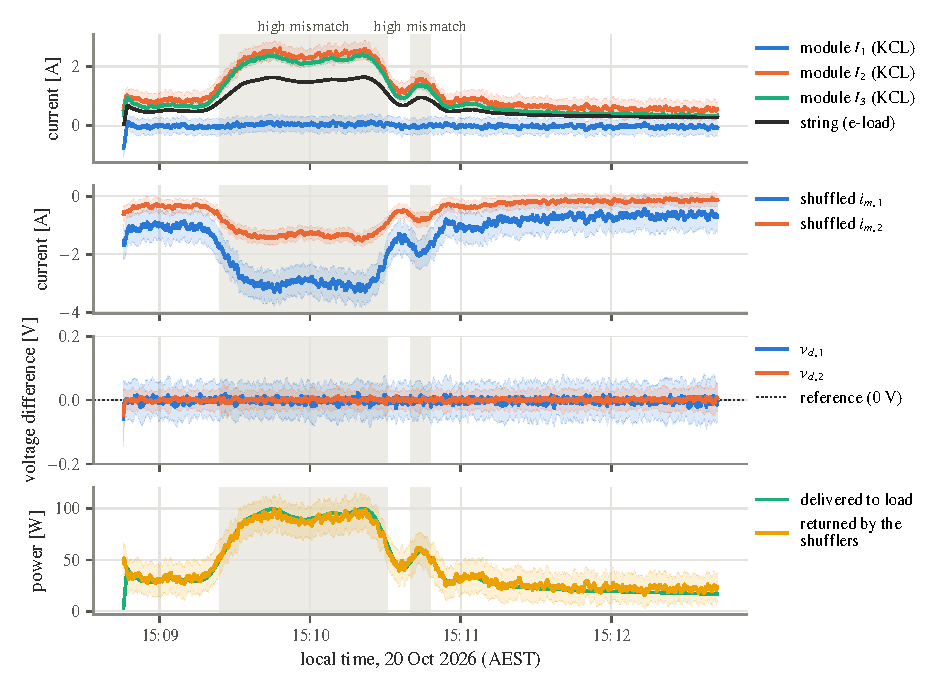
\includegraphics[width=\linewidth]{results/solar_S02}
  \caption[{Carpark string at peak sun, 200\,kHz closed loop, $k=0.1$ (S02, 20 Oct 2026)}]{Carpark string at peak sun, 200\,kHz closed loop, $k=0.1$ (S02, 20 Oct 2026): module currents rebuilt by KCL, shuffled currents, voltage differences and the power delivered to the 61\,V load and returned by the shufflers (1\,s means, $\pm1\sigma$ bands; shaded spans are the detected high-mismatch periods).}
  \label{fig:S02}
\end{figure}

The top module was shaded to almost zero current (a shirt over about a third of the panel): by KCL it carried $\approx 0\A$ in every solar window, while modules 2 and 3 carried up to 2.5\,A. The string current settled at the mean module current, as the model predicts, so the shufflers delivered the other two modules' power to the 61\,V load, up to 99\W{} during S02. A plain series string could not have supplied that load at all, so the energy returned equals the energy delivered: $E_{ret} = 10.6\Wh \approx E_{load}$ over the 36\,min (\cref{tab:T7solar}). \note{Confirm what happened to module 1 and phrase the energy return accordingly.} The measured ratio $E_{load}/E_{modules}$ of 99.2--100\,\% closes by construction, because $V_{M1}$ comes from the e-load and the module currents from KCL, so it is not a converter efficiency.

The weather was the main limitation. After 15:48 the sun was minimal ($P_{load}$ 2--13\,W), which allowed the gain sweep but not enough mismatch power to stress the loop. The closed-loop response to panel dynamics is therefore validated at low power, and otherwise rests on the models.

\subsection{Synthesising Results}
\label{sec:synthesis}
\Cref{fig:metrics} (and \cref{tab:T5s4}, \cref{app:synth}) compare the $+1\V$ reference step across the three models. The fitted time constant follows the design $1/(k\,2\pi\,150)$ at every gain scale: within 0.86--1.22$\times$ in the analytical model, 0.52--1.17$\times$ in QSPICE and 0.38--1.10$\times$ in the Simulink twin. The models drift faster than the design at high $k$, where the plant's own dynamics add to the integrator. Every one of these time constants is shorter than one 23\,ms telemetry frame, so the hardware cannot resolve the step response. What it does resolve agrees with the models: the DC gain (open-loop duty steps), zero steady-state error, a noise-limited residual, and closures within one frame.

\begin{figure}[htbp]
  \centering
  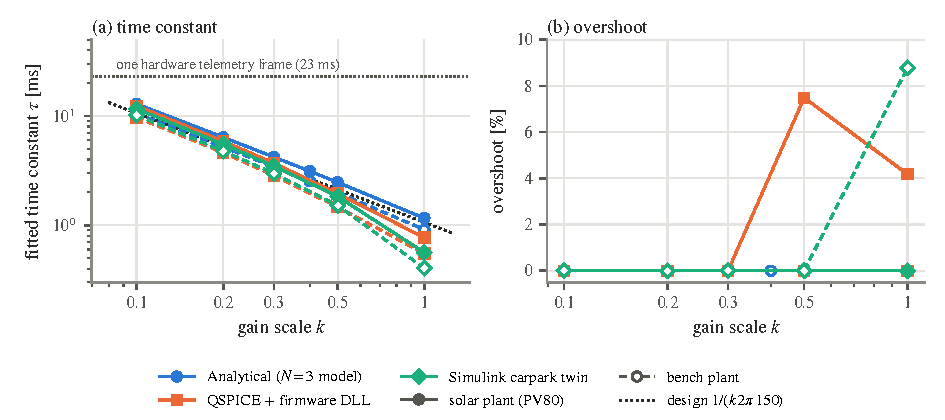
\includegraphics[width=\linewidth]{results/metrics_k}
  \caption[{$+1\V$ reference step on $\vd{}_{,2}$ (200\,kHz gain set) against gain scale}]{$+1\V$ reference step on $\vd{}_{,2}$ (200\,kHz gain set) against gain scale: (a) fitted time constant, with the first-order design and one hardware telemetry frame; (b) overshoot. Filled markers and solid lines are the solar plant, hollow markers and dashed lines the bench plant.}
  \label{fig:metrics}
\end{figure}


Most of the overshoot entries are zero (\cref{fig:metrics}(b), \cref{tab:T5s4}), and that is the design working rather than missing data. Because the controller inverts the DC gain, $MG$ is diagonal and each loop is an integrator acting on a plant of unit DC gain, which is a first-order closed loop, and a first-order response cannot overshoot. Overshoot needs the dynamics the design neglects: the 2\,kHz measurement filter, the one-tick delay of the 100\,$\mu$s sampling, and the plant's LC modes. These only matter once the loop's time constant falls to a few times their 0.1--0.3\,ms. That happens at $k \ge 0.5$ ($\tau \le 2\ms$), where QSPICE shows 7.5\,\% at $k = 0.5$ and 4.2\,\% at $k = 1$ on the solar plant and the Simulink twin 8.8\,\% on the bench plant at $k = 1$. The analytical model includes the filter but not the sampling delay, so it never overshoots.

Together these results support the gap claim: the same gain matrix decouples the voltage and current loops in an averaged model, in a switching model with sensing quantisation and dead time, and on the board at three switching frequencies. Where the phases disagree there is a reason. The Simulink twin is faster than the design at $k \ge 0.5$ because its averaged plant has no $R_{sw}$. QSPICE overshoots at high $k$ through the sampling delay and the filter. And the 300\,kHz gain set, identified at the bench operating point, loses margin on hardware earlier than the models suggest ($k = 0.6$ oscillation).

The risk, ethics and sustainability outcomes were met. There was no injury and no damaged component; U10's isolator was wired backwards before any testing. Every fault was latched by the firmware, all data stayed local on the Pi, and the string returned 10.6\Wh{} with one module producing nothing. The supervisor's feedback to push the controller algorithms into QSPICE, start rapidly testing early on in either simulink / qspice, support of learning from textbooks and papers and a strong emphasis on safety shaped the methods and direction of the project.
